\documentclass[11pt, a4paper]{article}

%Dimension de la page
%\usepackage[cm]{fullpage}
\usepackage[vmargin=2cm,hmargin=2cm]{geometry}


%permet l'utilisation des caractères accentués
\usepackage[utf8x]{inputenc}
\usepackage[T1]{fontenc}

%pour insérer des images 
\usepackage{graphicx}

%pour les formules mathématiques
\usepackage{amsmath, amsfonts}
\usepackage{amssymb, amsthm}

%typographie française
\usepackage[french]{babel}

%pour dessiner avec Latex
\usepackage{tikz}

%pour écrire les unités
\usepackage{siunitx}

%pour les en-têtes et pieds de page personnalisés (à gauche L, au centre C et à droite R)
\usepackage{fancyhdr}
\pagestyle{fancy}
\fancyhead[L]{
\includegraphics[scale=0.2]{insa.pdf} } %pour avoir le logo de l'insa à gauche (L), le fichier insa.pdf doit se trouver dans le même dossier que le fichier tex. 
\fancyhead[C]{TP-TD n°2  } % peut permettre d'indiquer un titre court au centre (C)
\fancyhead[R]{DAI Qinshu HUYNH Aline} % peut permettre d'indiquer le nom de l'auteur (R)
\renewcommand\headrulewidth{2pt}
\fancyfoot[C]{Page \thepage} % pour insérer le numéro de la page
\fancyfoot[R]{\today} % pour insérer la date  à droite (R)

%si l'on souhaite retirer l'une ou l'autre des parties des pieds de page ou en-tête, il suffit de "commenter" la ligne en ajoutant un signe pourcentage devant cette ligne. 

\usepackage{fancybox}% pour encadrer quelques mots à l'aide de la commande \fbox

\title{\textbf{TP-TD n°2 : Biprisme de Fresnel- Interférences de 2 ondes}}
\author{DAI Qinshu HUYNH Aline}
\date{\today}


\begin{document}

\maketitle
\thispagestyle{fancy}

\tableofcontents
\newpage

\section{Introduction}
Nous allons étudier le champ d’interférence du biprisme suivant 2 configurations différentes.

\bigskip

Liste du materiel:
\begin{itemize}
    \item une source Laser Nd :YAG type DPSS ($\lambda_{0}$ = 650 $n m$) équipé d’un objectif de microscope
    \item une lentille convergente L( $f = 100 mm$) 
    \item un Biprisme de Fresnel d'indice $n_{v}$ = 1,537 et d'angle $\alpha$ ($\approx$ 1°)
    \item un écran d'observation
    \item un détecteur matriciel ($1280\times1024$ pixels2, taille du pixel = 5,3 $\mu m$)
    \item 1 polariseur rectiligne P1

\end{itemize}

\section{Biprisme éclairé par une source ponctuelle à distance finie
    (ondes sphériques)}
\subsection{Méthode}
    \subsubsection{Montage}

    \begin{figure}[hbtp] %option h permet de mettre l'image à l'endroit indiqué
        \centering % permet de centrer l'image 
        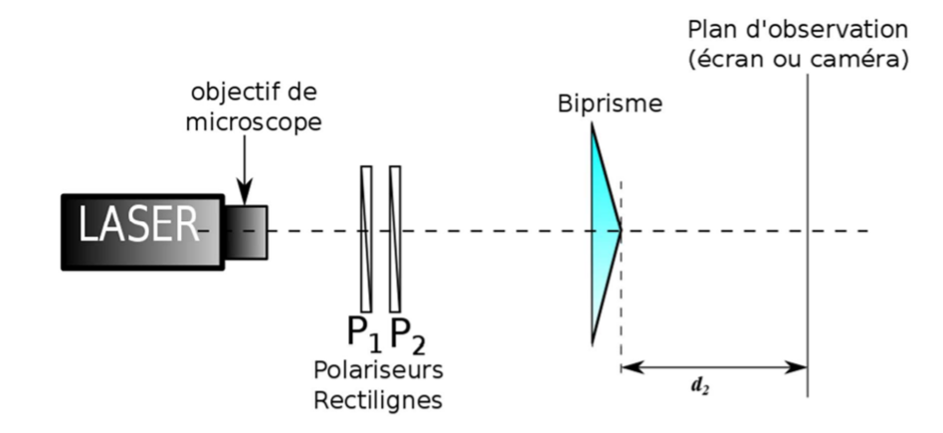
\includegraphics[width=0.75\textwidth]{schema1} % indiquer le nom du fichier de figure qui doit être enregistré dans le même dossier que le fichier tex, [scale=1] permet de régler la taille de la figure
        \caption{Schéma du dispositif expérimental permettant de visualiser les interférences entre 2 ondes sphériques} % permet de donner un titre à la figure
        \label{schema1}%donne le nom de référence de la figure qui peut être rappelée dans le texte à l'aide de \ref{insa}. Attention, il faut compiler deux fois pour que la numérotation des figures soit mise à jour dans le fichier pdf !
    \end{figure}
    \par
    La première configuration est celle représentée par la figure ci-dessus (Figure~\ref{schema1}) et correspond à un biprisme éclairé par une source ponctuelle à distance finie (onde sphérique).
\subsection{Résultats et Observations}
    On mesure l'évolution de l'interfrange en fonction de la distance entre le biprisme et la caméra, celle nous donne les valeurs suivantes:
    \begin{table}[htbp]
        \centering
    \begin{tabular}{|c|c|c|c|c|c|c|c|c|c|}
        \hline  
        \textit{d$_{2}$(cm)}&10&20&30&40&50&60&70&80&90\\
        \hline
        \textit{i (μm)}&69,96&94,3&118,7&143,2&170&193&221&238,5&268,2
        \\
        \hline 
    \end{tabular}
    \end{table}

    \begin{figure}[htbp] %option h permet de mettre l'image à l'endroit indiqué
        \centering % permet de centrer l'image 
        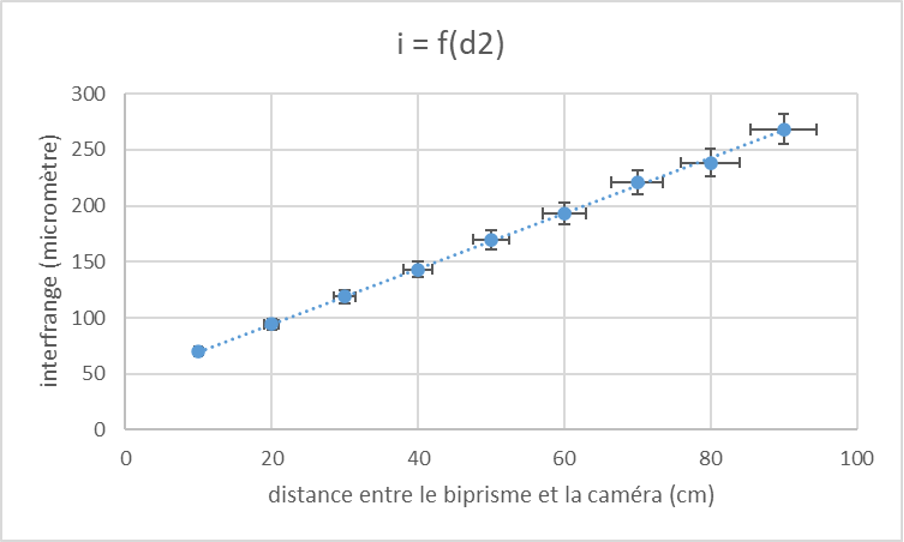
\includegraphics[width=0.75\textwidth]{courbe1} % indiquer le nom du fichier de figure qui doit être enregistré dans le même dossier que le fichier tex, [scale=1] permet de régler la taille de la figure
        \label{courbe1}%donne le nom de référence de la figure qui peut être rappelée dans le texte à l'aide de \ref{insa}. Attention, il faut compiler deux fois pour que la numérotation des figures soit mise à jour dans le fichier pdf !
    \end{figure}






\section{Biprisme éclairé par une source ponctuelle monochromatiqueplacée à l’infini}
\subsection{Méthode}
    \subsubsection{Montage}
    \begin{figure}[htbp] %option h permet de mettre l'image à l'endroit indiqué
        \centering % permet de centrer l'image 
        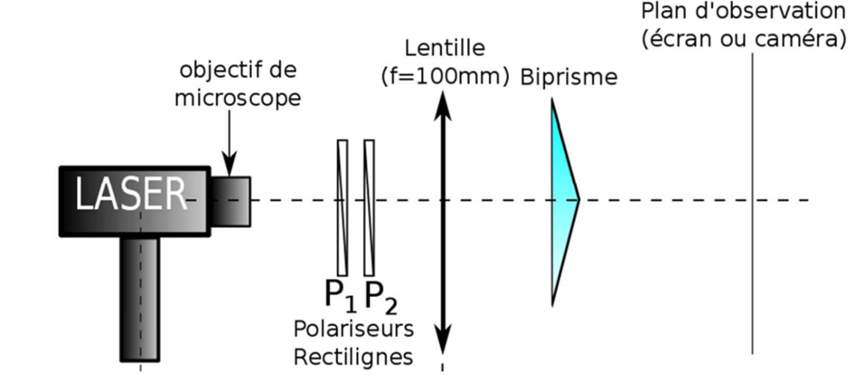
\includegraphics[width=0.75\textwidth]{schema2} % indiquer le nom du fichier de figure qui doit être enregistré dans le même dossier que le fichier tex, [scale=1] permet de régler la taille de la figure
        \caption{Schéma du dispositif expérimental permettant de visualiser les interférences entre 2 ondes planes} % permet de donner un titre à la figure
        \label{schema2}%donne le nom de référence de la figure qui peut être rappelée dans le texte à l'aide de \ref{insa}. Attention, il faut compiler deux fois pour que la numérotation des figures soit mise à jour dans le fichier pdf !
    \end{figure}
    Sans modifier le montage et les réglages précédents, on place une lentille L ($f=100 mm$) à la distance adéquate du pied portant le laser, en utilisant la cale en PVC gris mise à votre disposition (placer la cale entre la face avant de l’objectif et la monture de la lentille), et aligner son centre optique sur l’axe du faisceau laser.
    
\subsection{Résultats et Observations}
    \bigskip
    \begin{table}[htbp]
    \centering
    \begin{tabular}{|c|c|c|c|c|c|c|}
        \hline  
        \textit{d$_{2}$(cm)}&0
        &10
        &20
        &30
        &40
        &50
        \\
        \hline
        \textit{i (μm)}&43,40
        &44,50
        &44,50
        &41,34
        &40,29
        &39,00 
        \\
        \hline 
    \end{tabular}
    \end{table}
    \begin{figure}[htbp] %option h permet de mettre l'image à l'endroit indiqué
        \centering % permet de centrer l'image 
        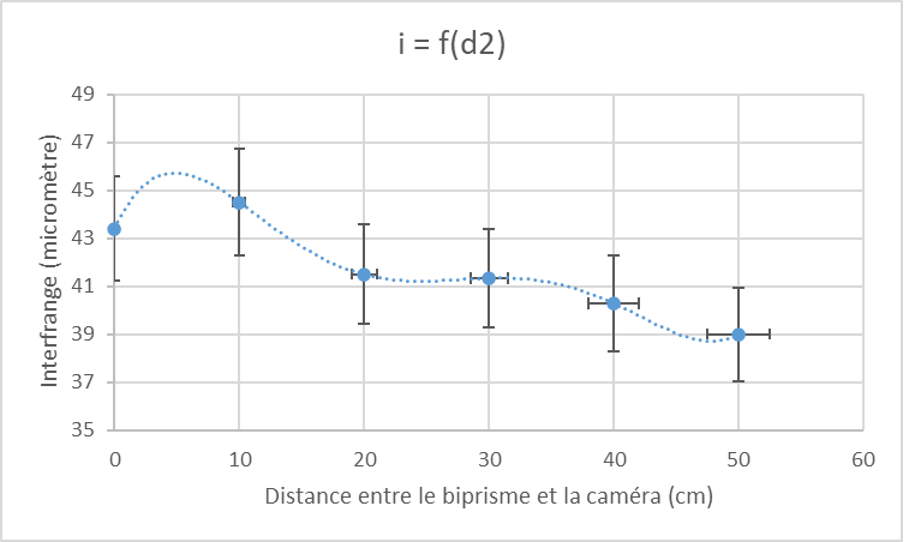
\includegraphics[width=0.75\textwidth]{courbe2} % indiquer le nom du fichier de figure qui doit être enregistré dans le même dossier que le fichier tex, [scale=1] permet de régler la taille de la figure
        \label{courbe2}%donne le nom de référence de la figure qui peut être rappelée dans le texte à l'aide de \ref{insa}. Attention, il faut compiler deux fois pour que la numérotation des figures soit mise à jour dans le fichier pdf !
    \end{figure}
\subsection{Etude du champ d’interference}

\section{INTERFERENCES EN LUMIERE BLANCHE (étude facultative)}
\subsection{Méthode}
    \subsubsection{Montage}
    \begin{figure}[htbp] %option h permet de mettre l'image à l'endroit indiqué
        \centering % permet de centrer l'image 
        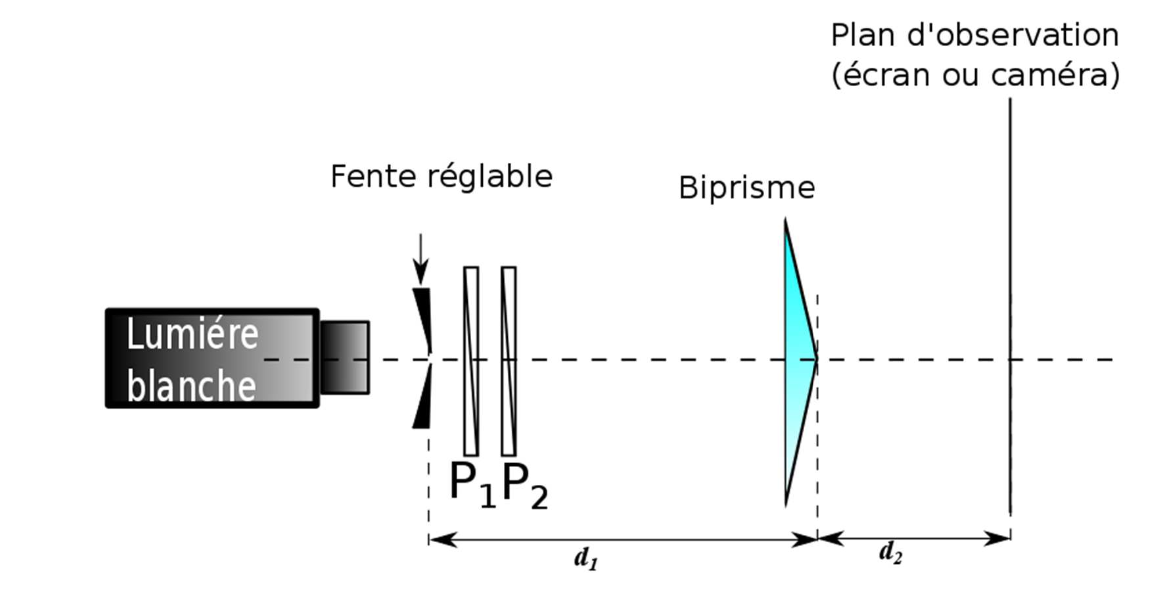
\includegraphics[width=0.75\textwidth]{schema3} % indiquer le nom du fichier de figure qui doit être enregistré dans le même dossier que le fichier tex, [scale=1] permet de régler la taille de la figure
        \caption{Schéma du dispositif expérimental permettant de visualiser les interférences en lumière blanche} % permet de donner un titre à la figure
        \label{schema3}%donne le nom de référence de la figure qui peut être rappelée dans le texte à l'aide de \ref{insa}. Attention, il faut compiler deux fois pour que la numérotation des figures soit mise à jour dans le fichier pdf !
    \end{figure}
    \subsection{Résultats et Observations}



\section{Discussion exploitation des résultats}


$\lambda_{0}=650nm$ 

$1 pixel=5,3 \mu m$
    \subsection{Incertitude}
    Sources d'incertitude :
    \begin{itemize}
        \item la mesure d'interfrange en pixel ;
        \item la lecture des distances sur le réglet.
        \end{itemize}

\section{Synthese TP-TD – comparaison theorie/experiences }
    \subsection{L’angle du biprisme $a$}
    \subsection{Conclusions}
    On peut également constater que pour une même valeur d'angle $\alpha$ du biprisme, la déviation augmente lorsque la distance $d$ entre le biprisme et l'écran diminue. Cela peut s'expliquer par le fait que plus la distance entre le biprisme et l'écran est grande, plus la lumière a de temps pour se propager avant d'arriver à l'écran, ce qui diminue la déviation.

    Enfin, on peut noter que les mesures expérimentales présentent des erreurs, ce qui peut s'expliquer par des facteurs tels que des imperfections dans la fabrication du biprisme, des fluctuations de l'intensité lumineuse ou des erreurs de mesure.



\end{document}

%%Contenu
    \bigskip

    Faire une liste non numérotée :
    \begin{itemize}
    \item premier item ;
    \item deuxième item.
    \end{itemize}

    \bigskip

    Faire une liste numérotée. 
    \begin{enumerate}
    \item Premier item. 
    \item Deuxième item.
    \end{enumerate}